
\documentclass[11pt,a4paper]{report}
%\pagestyle{headings} Might be interested in this

\usepackage{amsmath}                    % Extended math options
\usepackage{amssymb}                    % For special symbols, like collections Z,Q,R, etc.
\usepackage{graphicx}                     % To handle png and jpg figures
\usepackage{array}				% To handel complicated tables
\usepackage{caption}				% Allows captions with figures and tables
\usepackage[export]{adjustbox}		% To align images right and left 
\usepackage{indentfirst}			% Standard paragraph indent
\usepackage{wrapfig}				% For wrapping texts around figures and tables
\usepackage{capt-of}				% Caption extension
\usepackage{float}
\usepackage{geometry}

% Differential operator
\newcommand{\diff}{\ensuremath{\mathrm{d}}} 

% Super and subscript
\newcommand{\supsc}[1]{\ensuremath{^{\text{#1}}}}   % Superscript in text
\newcommand{\subsc}[1]{\ensuremath{_{\text{#1}}}}   % Subscript in text

\newcommand{\vt}[1]{\ensuremath{\boldsymbol{#1}}} % vector in correct lettertype
\newcommand{\mx}[1]{\ensuremath{\mathsf{#1}}}	  % matrix in correct lettertype

\newcommand{\omex}{\boldsymbol{\omega}_x}


\newcommand{\firstauth}[2]{\vspace{-\bibsepup}{\sc #1{,} #2}} %
\newcommand{\auth}[2]{{\sc #1{,} #2}} % use comment as \auth{Luppes}{R.}
\newcommand{\bibc}{{,} }              % separation between authors; no space!
\newcommand{\biba}{ and }             % last separation between authors
\newcommand{\noopsort}[1]{}           % correct bibliography order wrt year
\newlength{\bibsepup}                 % bibitems a bit higher \bibsepup;
\setlength{\bibsepup}{2.0mm}          % prevents too much spacing
\newcommand{\etal}{et al.}            % xspace would give too much space !

% End of the preamble.
% Beginning of body:

% Special word splittings
\hyphenation{back-slash}
\hyphenation{split-sings-uit-zon-de-ring}

\title{Tea with a Travelling Salesman:\\
	\large A Discussion of Genetic Algorithms}
\author{Karin Dijkstra, Anastasia Dryaeva, Rick Ploeg \& Oliver Strik\\
Propaedeutic Project: A11\\
Rijksuniversiteit Groningen}
\date{June 16 2017}
 

\begin{document}

\maketitle

\begin{abstract}
Abstract needs to be copied here!
\end{abstract}

\tableofcontents

% The various chapters
%\newpage 
\section{Introduction}

\par
The Travelling Salesman Problem (TSP) is a famous problem in combinatorial optimization, with the goal to minimize the total travel cost (be that time, distance, or fuel expenses) for a salesman who has to visit a finite number of cities and return to the starting point, given the costs associated with travelling from one city to another.

\par
At first the problem may appear uncomplicated and straightforward, however its simplicity is only an illusion. Although the exact origins of the TSP are unclear, it can be dated back to at least 1832, yet to this day, there has been no effective solution method found for a general case. In fact, a solution of this problem would resolve the infamous P vs. NP Millennium Prize problem. As a result, the Travelling Salesman Problem still remains one of the most intensely studied problems in computational mathematics and in the recent years has sparked interests in newer fields, such as computer science.

\par
Throughout the years, different methods and algorithms have been developed for the TSP. Many of the traditional methods involve heuristics such as Nearest Neighbor or Nearest Insertion, or relaxations, for example the Hungarian Algorithm. However, these do not necessarily give the optimal, and for the latter sometimes not even a feasible solution. Moreover, these methods become insufficient when the problem takes a larger scale. An example of a more advanced, newer method would be the application of a Genetic Algorithm. Genetic Algorithms (GAs) are algorithms designed to simulate natural evolution: they are based on the concept of “survival of the fittest”.

\par
This article will address the topic of applying a Genetic Algorithm to the Travelling Salesman Problem, focusing on the following question: “How do Genetic Algorithms perform when applied to the Travelling Salesman Problem?”. In order to provide an answer to this question, the TSP will be discussed in more detail in section \ref{IntroTSP}. After that, the general concept of a GA will be explained in section \ref{WisGA}, including an insight into the construction of such an algorithm for the TSP. In section \ref{SimpleTSP} the constructed GA will be applied to a small problem of 6 cities, where the efficiency of the algorithm will be evaluated in comparison to the traditional methods. Section \ref{largeTSP} will focus on investigating the performance of the GA on an expanded problem of 26 cities, including a discussion of the issues encountered, followed by a detailed analysis of the parameters within the constructed GA in section \ref{Analysis}. In the final section conclusions will be made, addressing the initial research question.




\section{What is a Genetic Algorithm?}
\par
\begin{figure}[h]
	\centering
		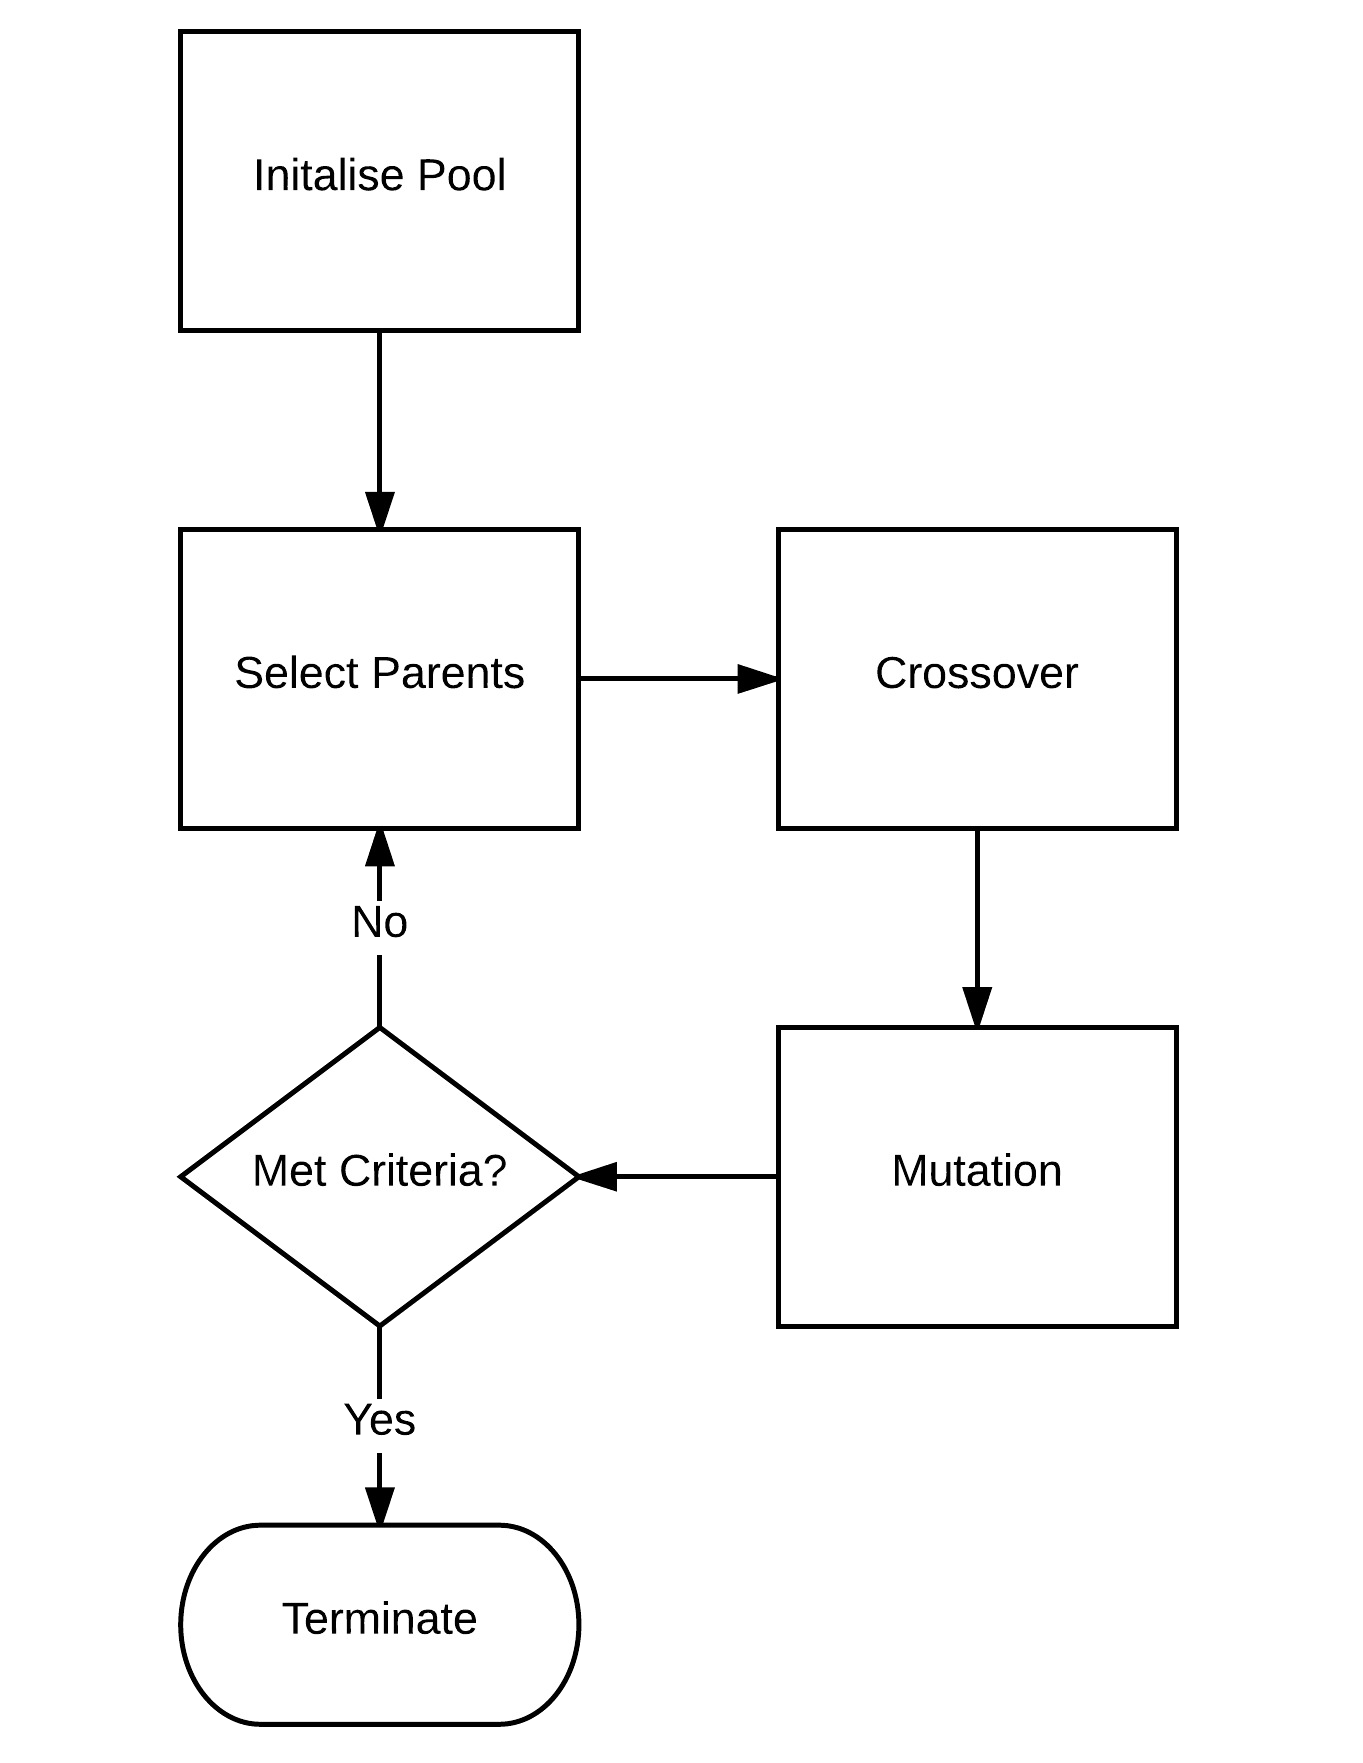
\includegraphics[width=0.5\textwidth]{GA_Structure}
	\caption{The basic structure of a Genetic Algorithm.}
	\label{struct}
\end{figure}
\noindent
A Genetic Algorithm is an algorithm that uses natural selection, or survival of the fittest, to find a solution to a problem. All Genetic Algorithms follow a similar, if not identical structure (figure \ref{struct}). However, the elements of this structure are highly customised for each specific application. Before going into detail about these elements, the concept of chromosomes and fitness must first be introduced.
\par
Chromosomes are one of the most important part of a GA, their only purpose is to store the potential solutions of the problem. How chromosomes store these solutions is up to the constructor of the GA, commonly however they are a single string that might represent a binary number, or possibly a list of the problems variables. Another important thing about chromosomes is their fitness. The fitness function of a GA describes how fit a particular problem is as a solution. How this fitness works, and how fitnesses are compared is again nearly entirely up to the constructor of the GA.


\section{Initialisation of the Pool}
\par
The first step in the execution of a Genetic algorithm is the generation of the pool. The pool is a collection of chromosomes that can be described as the "current generation". This pool is initialised by randomly generating chromosomes until the pool is filled, in the case of the research algorithm, this was done by shuffling the list of cities, thus eliminating the possibility of missing or having duplicate genes within the chromosome which was one of the constraints. The number of chromosomes in the pool is usually a fixed number, however adaptive pool sizing does exist (http://www.sciencedirect.com/science/article/pii/S2212671613000449) only fixed pool size was used in this research. 
\section{The Main Loop}
\par
This next section comprises the main body of the GA. Every time this loop is completed, a generation has passed. Through out the next sections, the methods used in the research algorithm will be used as examples.
\subsection{Parent Selection}\label{parents}
\par
Parent selection is the first step of each generation. The flow of Figure \ref{struct} suggests that all parents are selected before Crossover, however in reality it is easier and potentially more efficient to do both steps concurrently, thus you select two parents, breed them (Crossover) and repeat until a new pool is constructed.
\par
Parents can be selected in many ways, however usually the fitness of the parents is used in some way to select them. For example, in the research algorithm a method called roulette wheel selection was used (INSERT SOME REFERENCE HERE), in this method all chromosomes in the pool take up an area on a wheel proportional to the fitness of the chromosome. This created some issues as within the research algorithm as the fitness function returns the total distance of the chromosome, thus the smaller that distance the better it is. In order to get the correct probability of selection, the fitnesses needed to be 'inverted'. This was done with two equations: 
\[ inv = minFit + maxFit\]
\[ p = (inv - fitness)/totalInvFitness\]
Where $inv$ is the 'Inversion constant', $minFit$ is the smallest/best fitness in the pool, $maxFit$ is the largest/worst fitness in the pool, $p$ is the probability of selection, $fitness$ is the fitness of a chromosome, and $totalInvFitness$ is the sum of all inverted fitnesses in the pool.
\par
Using these equations, the probability of selection for each chromosome in the pool could be calculated, thus allowing for parents to be randomly selected from the pool using these probabilities.
\subsection{Crossover}\label{crossover}
\par
\begin{figure}[h]
\textit{Step 1:}
\[Parent\, 1: [0,3,\colorbox{green}{2,5,1},4]\]
\[Parent\, 2: [1,3,\colorbox{green}{5,0,4},2]\]
\[Child\, 1: [0,3,\colorbox{green}{2,5,1},4]\]
\[Child\, 2: [1,3,\colorbox{green}{5,0,4},2]\]
\textit{Step 2:}
\[Parent\, 1: [0,3,\colorbox{green}{2,5,1},4]\]
\[Parent\, 2: [1,3,\colorbox{green}{5,0,4},2]\]
\[Child\, 1: [-,3,\colorbox{green}{2,-,1},-]\]
\[Child\, 2: [-,3,\colorbox{green}{-,0,4},-]\]
\textit{Step 3:}
\[Parent\, 1: [0,3,\colorbox{green}{2,5,1},4]\]
\[Parent\, 2: [1,3,\colorbox{green}{5,0,4},2]\]
\[Child\, 1: [3,2,\colorbox{green}{-,-,-},1]\]
\[Child\, 2: [3,0,\colorbox{green}{-,-,-},4]\]
\textit{Step 4:}
\[Parent\, 1: [0,3,\colorbox{green}{2,5,1},4]\]
\[Parent\, 2: [1,3,\colorbox{green}{5,0,4},2]\]
\[Child\, 1: [3,2,\colorbox{green}{5,0,4},1]\]
\[Child\, 2: [3,0,\colorbox{green}{2,5,1},4]\]
\caption{Example of the crossover method used in the research algorithm. \label{fig:cross}}
\end{figure}
Crossover (also known as breeding) is when two chromosomes, called parents, are 'crossed' together in some way to produce one or more children. There are many ways of doing this, from slicing the parents in half and swapping the ends, to more complicated methods like the one used in the research algorithm shown in Figure \ref{fig:cross}.
\subsection{Mutation}
\par
\begin{figure}[h]
\textit{Step 1:}
\[Before: [0,3,\colorbox{green}{2},5,1,\colorbox{red}{4}]\]
\[After: [0,3,\colorbox{red}{4},5,1,\colorbox{green}{2}]\]
\caption{Example of the swap mutation used in the research algorithm \label{fig:mut}}
\end{figure}
Every child produced in Section \ref{crossover} has a chance of mutation, this is when the chromosome is subjected to a small but random change. In the case of the research algorithm, a specific form of mutation called swap mutation was used where two genes within the chromosome are randomly selected and then swapped, this is shown in Figure \ref{fig:mut}. Also, in the research algorithm, a chance of mutating multiple times was used with each subsequent mutation being less and less probable.
\section{Termination}
\par
The final step in the Genetic algorithm is termination. At the end of every generation, it is questioned whether the GA has met a specific criteria, if it has then the GA terminates and the best solution in the gene pool is the solution you finish with, otherwise it continues and begins a new generation.
\par
The criteria for termination can be nealy anything and are usually rather specific to the problem, however the are some generic ones, for example having found a solution that is better than a given solution or the simplest being having completed a given number of generations.
\section{The Research Framework}
\par
The Genetic Algorithm that was constructed for this research is divided into two components, the first being the Genetic Algorithm Framework (REFERENCE), and the second being a script which integrates with the framework.
The GAFramework is actually quite a simple program, it was designed for the research, however even though the research was specifically on the Traveling Salesman Problem, the GAF is capable of being used for any problem. It simply passes data to the scripts and provides the scripts some generic functionality such as a chromosome object and a loop function.
The script is the main bulk of the program as it is responsible for defining and solving a specific problem. The script constructed to solve the research problems was designed to be a generic script for Traveling Salesman Problems, when provided with a raw text file containing either a distance matrix or the coordinates for each city, it will proceed to solve the problem regardless of size. The script can also be given variables such as the size of chromosome pool, or the percentage of the pool to make elites. 


%\input{How does the Genetic Algorithm perform on a simple TSP?}
\chapter{How does the GA perform on a TSP of a larger scale?}
\section{Introduction}

\par
Considering the characteristics of a Genetic Algorithm, one can assume that they are not the standard method to use on problems of such a small scale as the problem discussed in Chapter 2, since manual or traditional methods can give the solution as well. GAs hold their real value in problems of a larger scale. Here they are capable of giving a feasible solution, where most other methods fail to give one or are just highly inefficient. The constructed GA has proved itself capable of dealing with a simple TSP containing six cities, but how does it perform on a TSP of a larger scale? This chapter will discuss the answer to that question, explaining the obstacles encountered along the way.

\par
The details of the TSP, such as the number of cities and their locations, will be addressed in the next section of this chapter. Then in the third section, the first performance of the GA on this TSP will be discussed. Since the total of possible tours was relatively low for the simple TSP, discussed in the previous chapter, the GA was capable of finding the optimal tour in every run. In this larger TSP however, the number of tours is significantly larger, which meant that the GA did not find the optimal tour in every run. This problem is known as premature convergence and is the topic of the fourth section. In the last section of this chapter a possible method to prevent premature convergence is discussed.

\section{A TSP containing 26 cities}
For this expansion it was decided to extend the problem to 26 cities. To make the problem more realistic, these 26 cities were selected to be located throughout the Netherlands. 

\begin{table} [t]
\parbox{0.4\textwidth}{

\begin{tabular}{l}
1 Amersfoort\\ 
2 Amsterdam\\
3 Apeldoorn\\
4 Arnhem\\
5 Assen\\
6 Breda\\
7 Den Haag\\
8 Den Helder\\
9 Eindhoven\\
10 Emmen\\
11 Enschede\\
12 Groningen\\
13 Haarlem\\
14 Heerenveen\\
15 Heerlen\\
16 ‘s-Hertogenbosch\\
17 Leeuwarden\\
18 Lelystad\\
19 Maastricht\\
20 Middelburg\\
21 Nijmegen\\
22 Rotterdam\\
23 Tilburg\\
24 Utrecht\\
25 Venlo\\
26 Zwolle
\end{tabular}

\label{26cities}
}
\qquad
\begin{minipage}[c]{0.6\textwidth} 
\footnotesize
\centering
\graphicspath{ {Afbeeldingen/} }
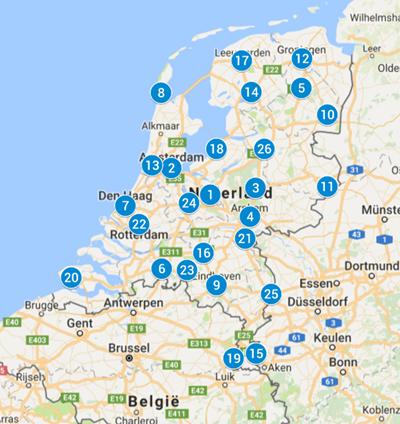
\includegraphics[width=1.2\textwidth, center]{26cities}
\captionof{figure}{26 cities, marked on the map of the Netherlands}
\label{map1}
\end{minipage}
\end{table}

\newpage
\par
The 26 cities are listed in alphabetical order together with a map of the Netherlands (figure \ref{map1}), that marks all of their locations. The objective is thus to find the shortest route that visits all of these cities and returns to the starting point afterwards. The total number of possible tours here is calculated by equation: %future reference needed
\[n = \frac{(26-1)!}{2} =  7.755605e+24\]
This number is significantly larger than the 60 possible tours for the simple TSP, discussed in chapter 2. This is then also the reason why most other methods fail to give a solution or are just inefficient. The manual methods and traditional methods, discussed in the previous chapter, are excellent examples. The Hungarian Algorithm already took 2 hours to perform on a TSP, containing only six cities and even though it did give the optimal solution in the end, it is highly inefficient to apply to this TSP because of the time it would take. In addition, this algorithm is a manual method, which makes it susceptible for human errors. The BIP also fails to give a solution, because the number of integer variables exceeds the limit of the Microsoft Excel linear solver. Even without this limit of variables, a BIP would take a long time to construct, considering all the possible subtours that would have to be added to the program as constraints in order to make sure that the resulting tour meets the criteria, set by the TSP. All of these subtours have to be excluded by manually adding these constraints, which makes the BIP timewise an inefficient method.Therefore it is necessary to turn to other methods, such as Genetic Algorithms. Even though they are not bound to give the optimal solution, they are at least capable of giving a suitable tour that meets the criteria, set by the TSP.

\section{The performance of the GA}

\par
The first observation, when the GA was applied to the expanded TSP, was that the time for one run of the program had increased. Depending on the settings, such as the number of generations and the poolsize, the program now takes approximately a minute. Since one chromosome now consists of not 6, but 26 genes, it makes sense that the time for one run increased. One minute is still a relatively short amount of time to find a solution. Besides the short time, another benefit is that the GA did not need reconstructing in order to be applied to this expanded TSP. Because of the way the basic structure was programmed, this GA can be applied to any TSP, that sparks your interest given that you provide the necessary data, which consists of the number of cities and their distances to each other. For other methods, like the Hungarian Algorithm or the BIP, this does not hold. 

%\input{Analysis}
%\input{Discussion, issues, further research and conclusion}
%\begin{thebibliography}{9}
\bibitem{Google}
Google.
\textit{Google Maps} [Google Maps distances].
Retrieved: May 19, 2017.

\bibitem{Congress}
L. Juan, C. Zixing, and L. Jianqin.
"Premature convergence in genetic algorithm: Analysis and prevention based on chaos operator."
\textit{Proceedings of the 3rd World Congress on Intelligent Control and Automation} 2010: 495-499.

\bibitem{Popdiv}
Y. Leung, Y. Gao, and Z. Xu.
"Degree of Population Diversity - a Perspective on Premature Convergence in Genetic Algorithms and Its Markov Chain Analysis." \textit{IEEE Transactions on Neural Networks}, 8(5) (1997): 1165-176. 

\bibitem{Operations}
J.D.C. Little, K.G. Murty, D.W. Sweeney and C. Karel. "An algorithm for the traveling salesman problem." \textit{Operations Research}, Vol. 11 (1963): 972–989.

\bibitem{Basics}
M. Mitchell.
\textit{ An introduction to genetic algorithms.} Cambridge MA: MIT Press, 1998.

\bibitem{Premconvergence}
H. M. Pandey, A. Chadhary and D. Mehrota.
"A Comparative Review of Approaches to Prevent Premature Convergence in GA." \textit{Applied Soft Computing} 24 (2014): 1047-1077. 

\bibitem{Online}
D. Pardini.
[\textit{TSP optimum tour}], November 9 2015. Retrieved: June 5, 2017. Available: https://otimizacaonapratica.wordpress.com/2015/11/09/o-problema-do-caixeiro-viajante/.

\bibitem{populationsize}
B.R. Rajakumar and Aloysius George. "APOGA: An Adaptive Population Pool Size Based Genetic Algorithm." \textit{AASRI Procedia} 4 (2013): 288-96.

\bibitem{Thesis}
J. P. Ryan.
\textit{An algorithm for the solution of a traveling salesman problem to minimize the average time to demand satisfaction} [Unpublished master's thesis]. Texas AM University, 1992. Retrieved: June 3, 2017.
\end{thebibliography}




\end{document}

